\documentclass[12pt]{article}

%packages
\usepackage{fancyhdr}
\usepackage[margin=1in]{geometry}
\usepackage[utf8]{inputenc}
\usepackage{listings}
\usepackage{booktabs}
\usepackage{enumitem}
\usepackage{pdfpages}
\usepackage{graphicx}
\usepackage{listings}
\usepackage{xcolor}
\usepackage{rotating}
\usepackage{subcaption}
\usepackage{float}
\usepackage{amsmath}

%fancyheadr fix
\setlength{\headheight}{15pt}

%commands to lslistings
\lstset{
    basicstyle=\ttfamily\small,
    breaklines=true,     
    breakatwhitespace=true,
    frame=single,
    numbers=left,
    numberstyle=\tiny,
    columns=fullflexible,
    keepspaces=true
}


%title info
\newcommand{\doctitle}{STA 5635 HW 10}
\newcommand{\name}{Palmer Swanson}
\newcommand{\docdate}{\today}

%document
\begin{document}

\begin{center}
    {\Large \doctitle}\\[6pt]
    {\name}\\[3pt]
    {\docdate}
\end{center}
%\vspace{12pt}

%part a, the clustering results
\begin{figure}[htbp]
    \centering

    \begin{subfigure}{0.45\textwidth}
        \centering
        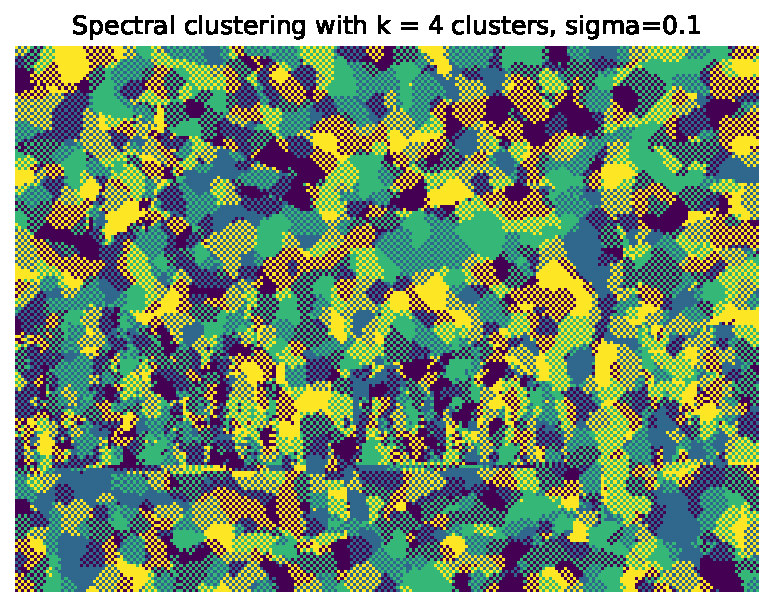
\includegraphics[width=0.85\linewidth]{../figures/clusters_k4_sigma0.1.pdf}
        \caption{$k=4$, $\sigma=0.1$}
    \end{subfigure}
    \hfill
    \begin{subfigure}{0.45\textwidth}
        \centering
        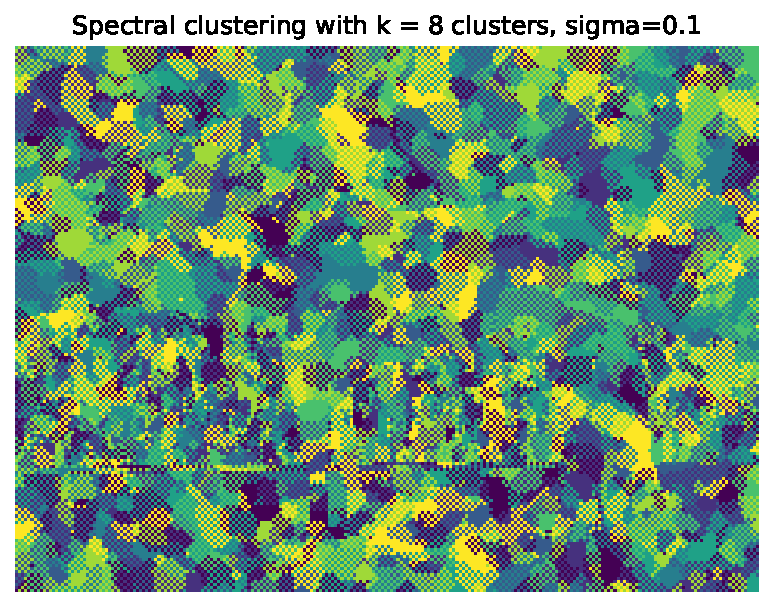
\includegraphics[width=0.85\linewidth]{../figures/clusters_k8_sigma0.1.pdf}
        \caption{$k=8$, $\sigma=0.1$}
    \end{subfigure}

    \vspace{0.5em}

    \begin{subfigure}{0.45\textwidth}
        \centering
        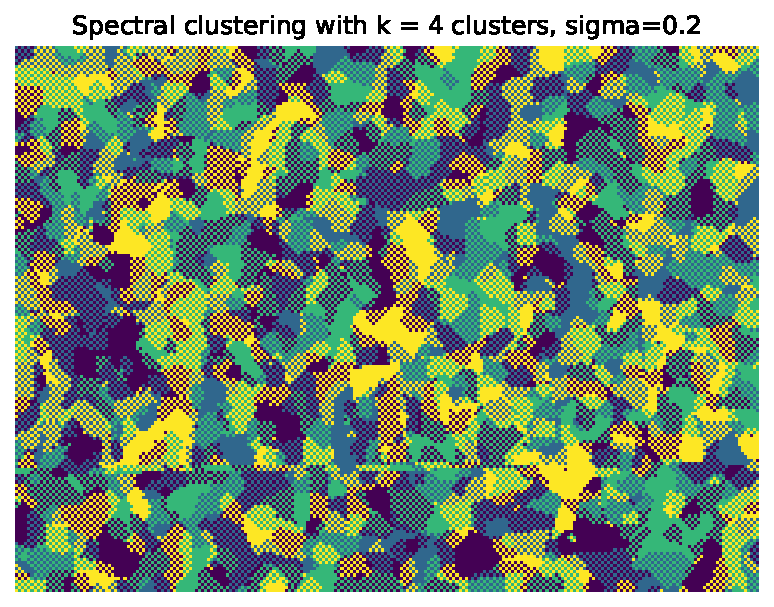
\includegraphics[width=0.85\linewidth]{../figures/clusters_k4_sigma0.2.pdf}
        \caption{$k=4$, $\sigma=0.2$}
    \end{subfigure}
    \hfill
    \begin{subfigure}{0.48\textwidth}
        \centering
        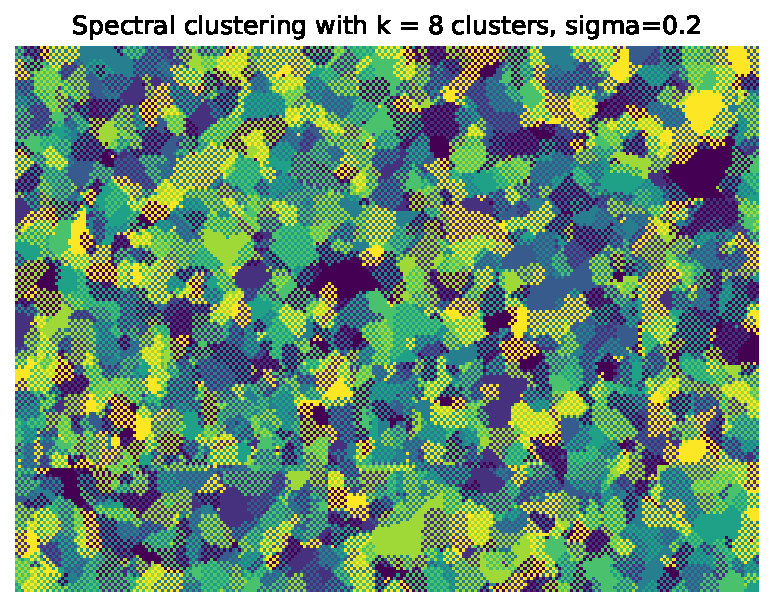
\includegraphics[width=0.85\linewidth]{../figures/clusters_k8_sigma0.2.pdf}
        \caption{$k=8$, $\sigma=0.2$}
    \end{subfigure}

    \vspace{0.5em}

    \begin{subfigure}{0.45\textwidth}
        \centering
        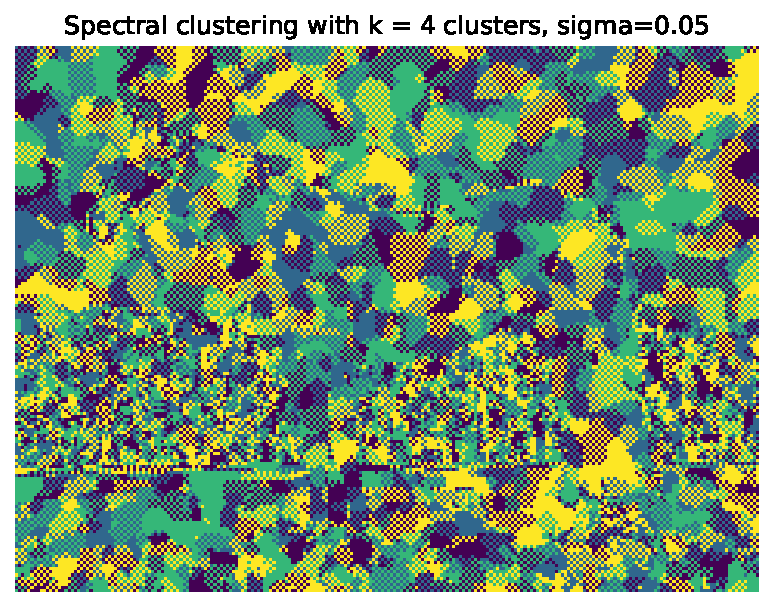
\includegraphics[width=0.85\linewidth]{../figures/clusters_k4_sigma0.05.pdf}
        \caption{$k=4$, $\sigma=0.05$}
    \end{subfigure}
    \hfill
    \begin{subfigure}{0.45\textwidth}
        \centering
        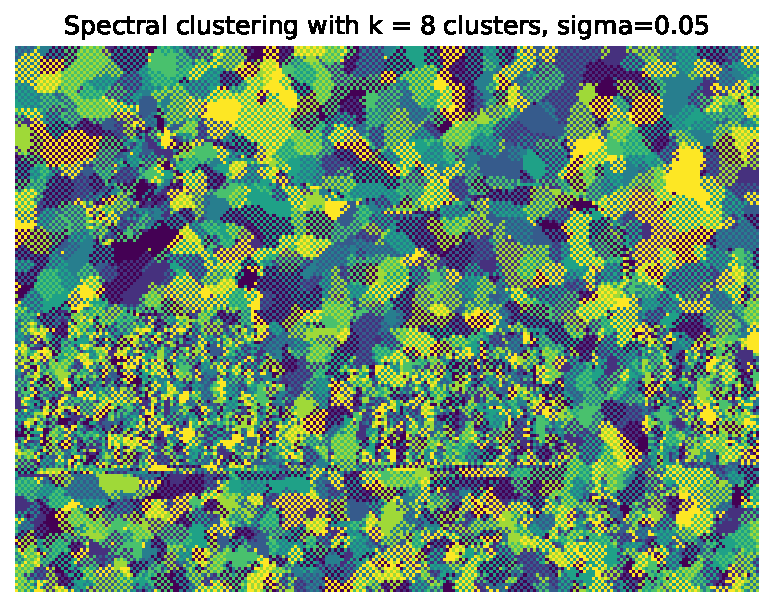
\includegraphics[width=0.85\linewidth]{../figures/clusters_k8_sigma0.05.pdf}
        \caption{$k=8$, $\sigma=0.05$}
    \end{subfigure}

    \caption{Spectral clustering results for different values of $k$ (clusters) and $\sigma$.  Part a.}
    \label{fig:spectral_clusters}
\end{figure}

%part b, the mean of the RGB values
\begin{figure}[htbp]
    \centering

    \begin{subfigure}{0.45\textwidth}
        \centering
        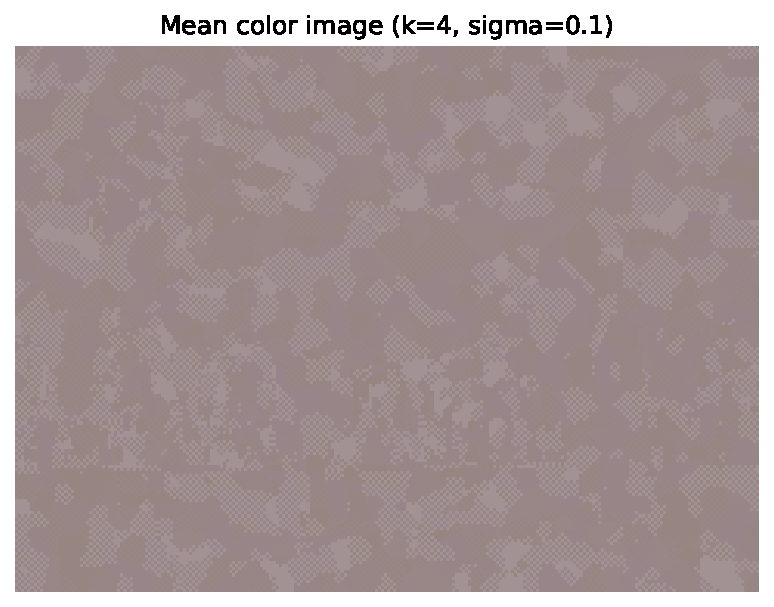
\includegraphics[width=0.85\linewidth]{../figures/mean_k4_sigma0.1.pdf}
        \caption{$k=4$, $\sigma=0.1$}
    \end{subfigure}
    \hfill
    \begin{subfigure}{0.45\textwidth}
        \centering
        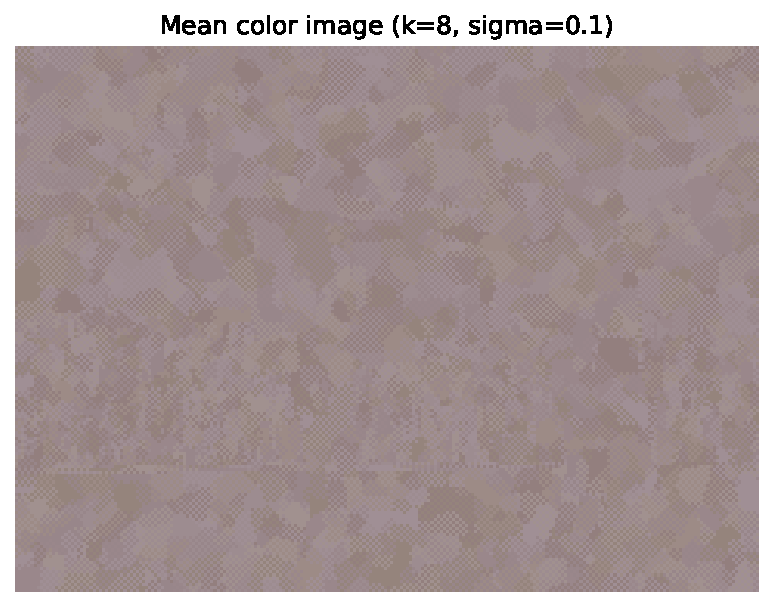
\includegraphics[width=0.85\linewidth]{../figures/mean_k8_sigma0.1.pdf}
        \caption{$k=8$, $\sigma=0.1$}
    \end{subfigure}

    \vspace{0.5em}

    \begin{subfigure}{0.45\textwidth}
        \centering
        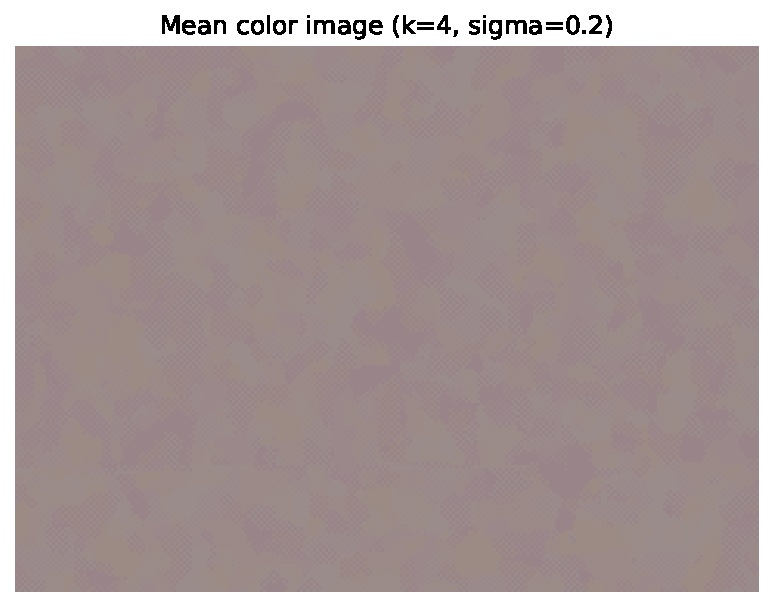
\includegraphics[width=0.85\linewidth]{../figures/mean_k4_sigma0.2.pdf}
        \caption{$k=4$, $\sigma=0.2$}
    \end{subfigure}
    \hfill
    \begin{subfigure}{0.45\textwidth}
        \centering
        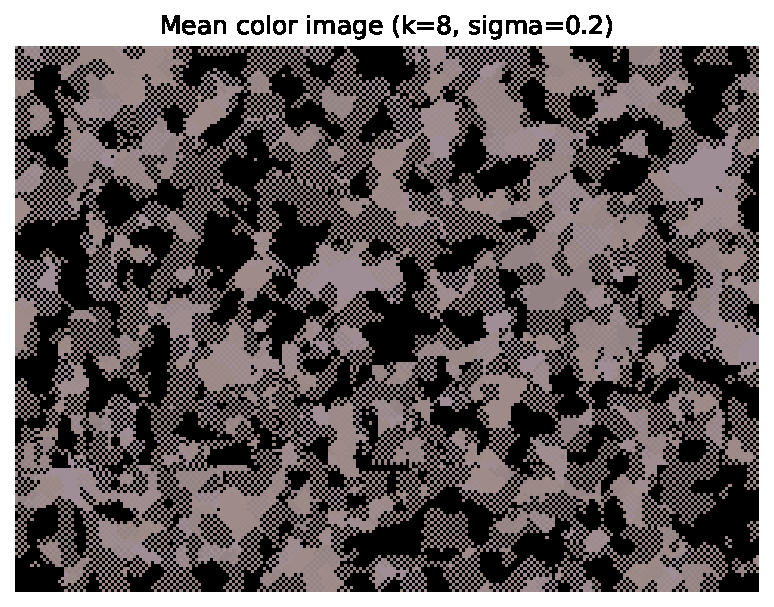
\includegraphics[width=0.85\linewidth]{../figures/mean_k8_sigma0.2.pdf}
        \caption{$k=8$, $\sigma=0.2$}
    \end{subfigure}

    \vspace{0.5em}

    \begin{subfigure}{0.45\textwidth}
        \centering
        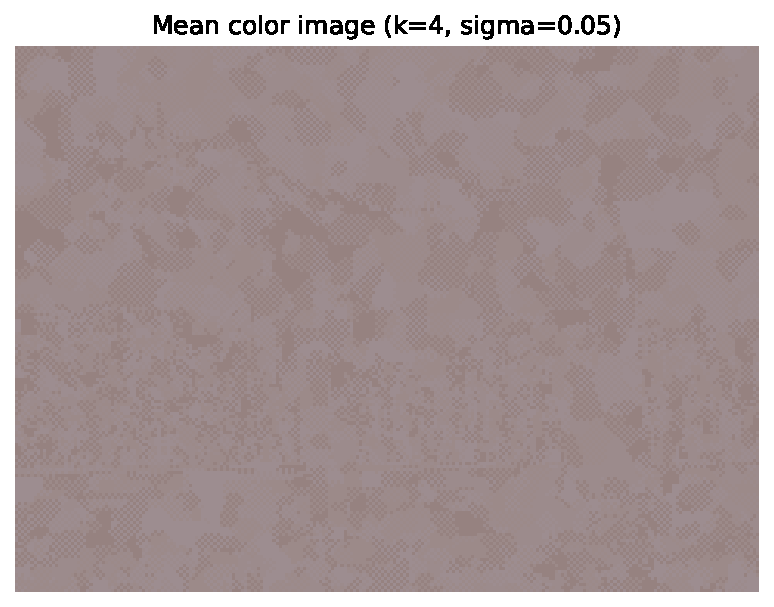
\includegraphics[width=0.85\linewidth]{../figures/mean_k4_sigma0.05.pdf}
        \caption{$k=4$, $\sigma=0.05$}
    \end{subfigure}
    \hfill
    \begin{subfigure}{0.45\textwidth}
        \centering
        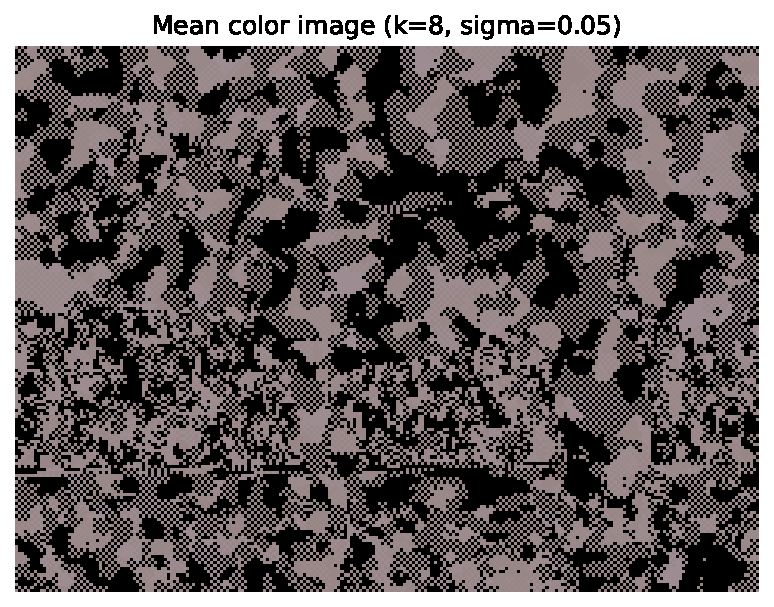
\includegraphics[width=0.85\linewidth]{../figures/mean_k8_sigma0.05.pdf}
        \caption{$k=8$, $\sigma=0.05$}
    \end{subfigure}

    \caption{Mean-color images for different values of $k$ and $\sigma$.  Part b}
    \label{fig:mean_color_images}
\end{figure}

% \newpage
% \newpage
% %adding code
% \appendix
% \section*{Code}
% \lstinputlisting[language=Python]{../code/hw09.py}

\end{document}